\chapter{Hierarchical Control for Head-to-Head Racing} 
% \epigraph{\flushright The Turn}{}
\epigraph{\flushright The second act is called ``The Turn". The magician takes the ordinary something and makes it do something extraordinary.}{Christopher Priest}
\label{chapter:hier}
\section{Hierarchical Control Design}
% \begin{figure}
%   \centering
%   \includegraphics[height=0.5\textheight]{Figures/ControlStructureVertical.png}
%   \caption{The continuous dynamic game (top) transformed into the high-level discrete game (middle). The discrete game solution created by the high-level planner (highlighted in green) is tracked by the low-level planner (bottom).}
%   \label{fig:overall_control}
% \end{figure}
\begin{figure*}
  \centering
%   \includegraphics[width=\textwidth]{Figures/FormulationBreakdown.png}
    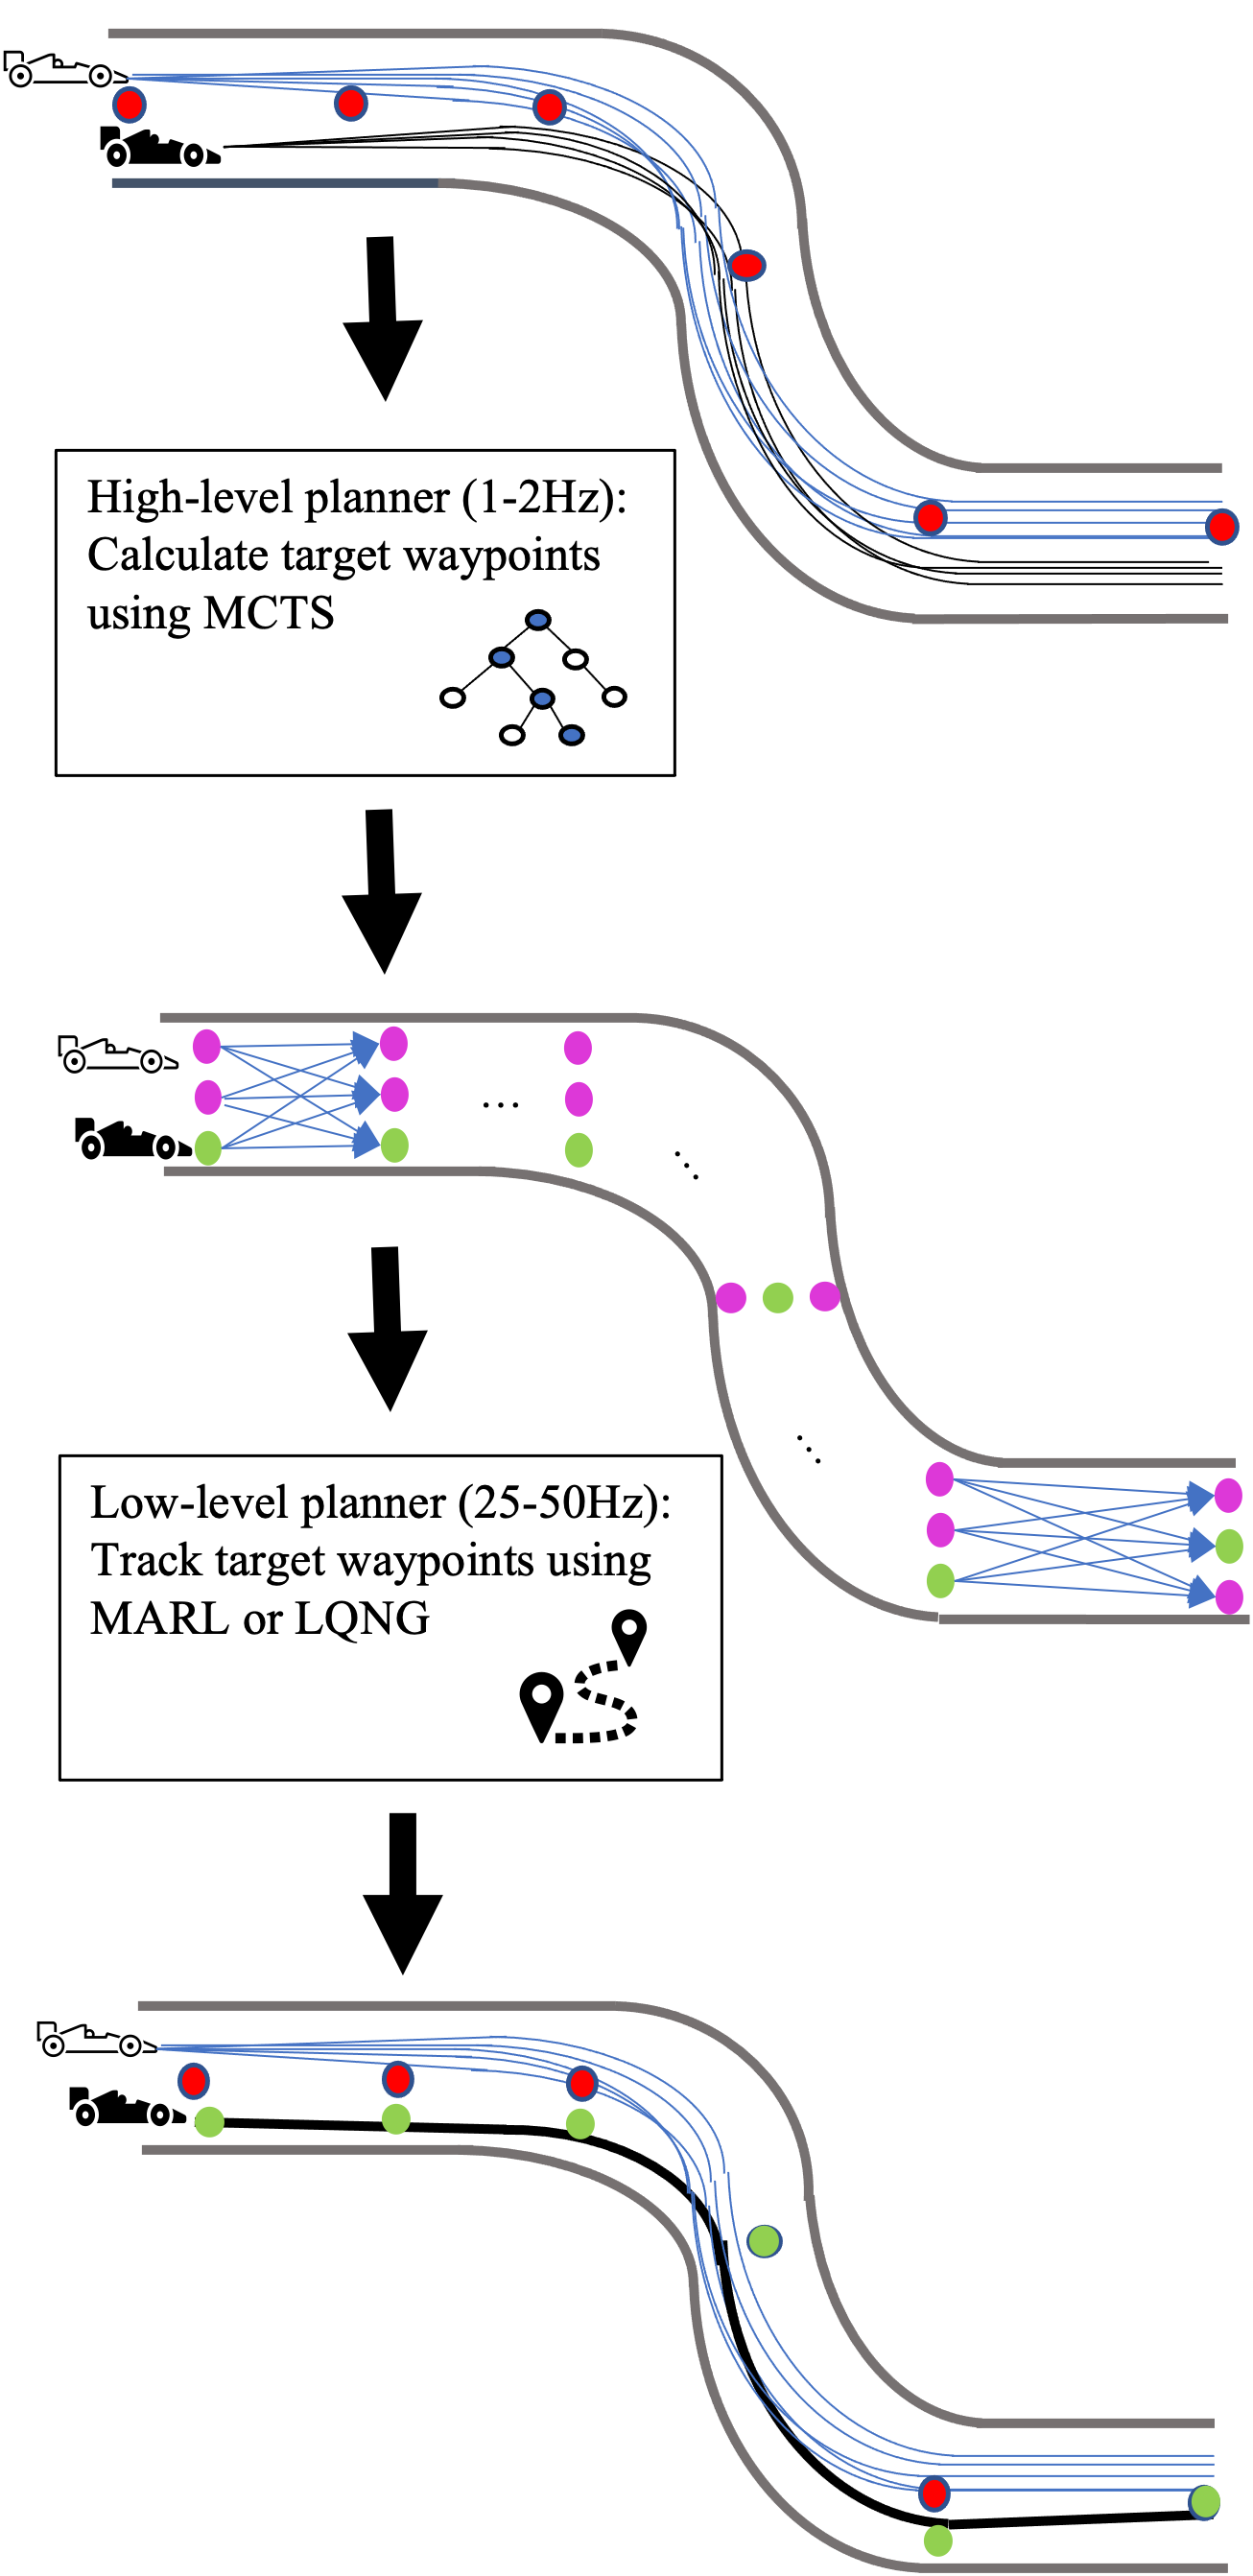
\includegraphics[height=0.8\textheight]{Figures/FormulationBreakdownVert.png}
  \caption[Hierarchical Control Architecture]{The uncountably infinite trajectories of the general game (top) discretized by the high-level planner (middle). The sequence of target waypoints calculated by the high-level planner (in green) is tracked by the low-level planner (bottom) and converges to a continuous trajectory (in black).}
  \label{fig:overall_control}
\end{figure*}
Traditional optimization-based control methods cannot easily be utilized for the general multi-agent racing game formulated with realistic safety and fairness rules in Section \ref{section:genform}. The rules involve nonlinear constraints over both continuous and discrete variables, and a mixed-integer non-linear programming algorithm would be unlikely to run at rates of \SI{25}{\hertz}-\SI{50}{\hertz} for precise control. This inherent challenge encourages utilizing a method such as deep reinforcement learning or trying to solve the game using short horizons. 

However, we propose a hierarchical control structure involving two parts that work to ensure all of the rules are followed while approximating long-term optimal choices. The high-level planner constructs a discrete game approximation of the original formulation where all of the discrete rules are naturally encoded. The solution provided by the high-level planner is a series of discrete states (i.e waypoints) for each player, which satisfies all of the rules. Then, the low-level planner solves a simplified version of the racing game with an objective putting greater emphasis on tracking a series of waypoints and smaller emphasis on the original game-theoretic objective and a simplified version of the rules. Therefore, this simplified formulation can be solved by an optimization method in real-time or be trained in a neural network when using a learning-based method. 

This method assumes that if the series of waypoints produced by the high-level planner is guaranteed to follow the rules, then the control inputs generated by the waypoint tracking low-level planner will also satisfy the rules of the original game when applied to the actual underlying system. Figure \ref{fig:overall_control} visualizes the overall control architecture.

\subsection{High-Level Planner}
The high-level planner constructs a turn-based discrete, dynamic game that is an approximation of the general game outlined in Equations \eqref{eq:gen_obj}-\eqref{eq:gen_lane_lim}. We formulate the high-level game using the model discussed in Chapter \ref{chapter:synthesis} using a receding horizon of checkpoints near the player to have a reasonable shot at solving the game for real-time control. However, our choice of horizon extends much further into the future than an MPC-based continuous state/action space controller can handle in real time \cite{Wang2019}. In the following subsections, we briefly summarize how the discrete game constructed and how we use Monte Carlo tree search to approximately solve the game.

\subsubsection{Discrete Game Construction}
% Describe High-Level Game (states, transitions, rewards)
Constructing our discrete game relies primarily on forming the initial states of the players. Given the initial states, the remaining feasible states and components of the game arise naturally by following the dynamics in Section \ref{section:discdyn}. 

To select the initial state of the game, we first construct a subset of the overall set of players based on how far away they are from the ego player. Because the discrete game is fixed to a finite horizon of checkpoints, the players that would likely have a significant impact on an ego player's trajectory are those who are within some local vicinity of the ego player. Using the set of local players, the initial checkpoint of the game is selected to be the one that the furthest forward player in the local vicinity has passed, and the target checkpoint is a fixed count ahead of the initial checkpoint. 

The continuous components of the players' states are projected into their discrete representations as described in Section \ref{section:discstate}. Initial state values for speed, velocity, tire wear, lane ID, and ``recent" lane changes are easily extracted from their continuous state. However, because some players may not have reached the selected initial checkpoint of the discrete game, their initial time state must be estimated. We assume each player has access to the times at which each checkpoint was passed by each of the other players. Using the time at the last checkpoint passed by all players, the initial time state is set to 0 for the furthest forward player, and the remaining players' initial time states are set to max of 0 and difference in their times at the last passed checkpoint with respect to the furthest forward player. Figure \ref{fig:disc_construct} shows this initial state construction process applied to a 4 player situation.

As mentioned, given the initial states of the players, the remaining construction of the game follows directly from the other parts of the formulation. The objective is the same as described in Section \ref{section:discobj}, but we do not use model checking software/algorithms to solve the game for our hierarchical controller. Table \ref{table:discrete_exp_summary} shows that it takes about 3-4 minutes to solve a single instance using state-of-the-art model checking software. We expect to run the high-level planner at \SI{1}{\hertz} to \SI{2}{\hertz}.

\subsubsection{Monte Carlo Tree Search}
Although the discrete game is much simpler than the original formulation, the state space still grows exponentially as the number of actions and players increases. Therefore, we cannot rely the model checking methods for real-time control. In order to produce a reasonable strategy for the discrete game in real-time, we use the Monte Carlo tree search (MCTS) algorithm to approximate the solution to our game \cite{mcts}. Our implementation of the MCTS algorithm is the same as the original with one exception: instead of sampling the feasible action set uniformly in the simulation step, we use a heuristic to bias our sampling towards those actions deemed more likely to be realistic or optimal. Recall that the actions available at each state is a set $A$ of pairs of lane ID and velocity. We sort the action set using following characteristics of each action in the priority as listed:
\begin{enumerate}
    \item Ascending by the elapsed time calculation \eqref{eq:time_update}
    \item Descending by target velocity of the action
    \item Ascending by absolute difference between target lane ID and current lane ID
    \item Ascending by the difference between target lane ID and the lane ID of the optimal racing line
\end{enumerate}
Once the actions are sorted, we randomly sample an index to select an action from the sorted set using following calculation:

\begin{equation}
    \text{action index} = [\min(|x|, |A|)], \quad
     x \sim \mathcal{N}(0, \frac{|A|}{6})
\end{equation}

Though the reward function is the same as the discrete formulation, we normalize it between 0 and 1 when calculating the upper confidence bound scoring in the MCTS algorithm. The solution produced by applying MCTS to our discrete game is a series of waypoints in the form of target lane IDs (which are mapped back to locations on track) and the target velocities at each of the locations. These waypoints are generated for all players considered in the discrete game and are selected assuming everyone selects their optimal choice. The top and middle of Figure \ref{fig:overall_control} visualize the original, continuous formulation expanded into a discrete game with the target waypoints highlighted in green.  

\subsection{Low-Level Planner}
% Describe Simplified waypoint Following Game
The low-level planner is responsible for producing the control inputs, so it must operate at even higher frequencies than the high-level planner. Because we have a long-term plan in the form of target waypoints from the high-level planner, we formulate a reduced version of the original game for our low-level planner. The low-level game is played over a shorter horizon compared to the original game of just $\delta$ steps in $\hat{\mathcal{T}} = \{1, ..., \delta\}$. We assume that the low-level planner for player $i$ has received $k$ waypoints, $\psi^i_{r^i_{1}}, ..., \, \psi^i_{r^i_{1} + k}$, from the high-level planner. Lastly, we also access player $i$'s last passed checkpoint $r^i_*$. 
% Table \ref{tab:ll_symbols} includes the additional parameters referenced in the simplified formulation.

The low-level objective involves two components. The first is to maximize the difference between its own checkpoint index and the opponents' checkpoint indices at the end of $\delta$ steps. The second is to minimize the tracking error, $\eta^i_y$, of every passed waypoint $\psi^i_{r^i_{1}+y}$. The former component influences the player to pass as many checkpoints as possible, which suggests reaching $c_\tau$, the final checkpoint, as quickly as possible. The latter influences the player to be close to the high-level planner's target waypoints when passing each of the checkpoints. The objective also includes a multiplier $\alpha$ that balances the emphasis of the two parts. The objective is written as follows:
% Low-Level Formulation

\begin{equation} \label{eq:ll_obj}
    \min_{u^i_{1}, ..., u^i_{\delta}} (\sum^N_{j \neq i}r^j_{\delta} - (|N|-1) r^i_{\delta}) + \alpha \sum_{c={r^i_{1}}}^{{r^i_{1}}+k} \eta^i_c
\end{equation}

The players' continuous state dynamics, calculations for each checkpoint, and constraints on staying within track bounds  are effectively the same as the original formulation \eqref{eq:ll_dyn}-\eqref{eq:ll_pos_dist}. 

\begin{equation} \label{eq:ll_dyn}
    x^j_{t+1} = f(x^j_{t}, u^j_t), \quad \forall \;\; t \in \hat{\mathcal{T}}, j \in N
\end{equation}
\begin{equation} \label{eq::ll_pos}
    r^j_{t+1} = p(x^j_{t+1}, r^j_t), \quad \forall \;\; t \in \hat{\mathcal{T}}, j \in N
\end{equation}
\begin{equation} \label{eq::ll_pos_init}
    r^j_{1} = r^j_*, \quad \forall\;\; j \in N
\end{equation}
\begin{equation} \label{eq:ll_pos_dist}
    q(x^m_{t}) \leq w, \quad \forall \;\; t \in \hat{\mathcal{T}}, j \in N
\end{equation}

The collision avoidance rules are simplified to just maintaining a minimum distance $s_0$ as the high-level planner would have already considered the nuances of rear-end collision avoidance responsibilities defined in constraint \eqref{eq:gen_coll_avoid} from the general formulation. Therefore, we require the following constraint to hold for all $t \in \mathcal{T}$, $j \in N$, and $k \in N \setminus \{j\}$:
\begin{equation} \label{eq:ll_coll_avoid}
    d(x^j_{t}, x^k_t) \geq s_0
\end{equation}

Finally, we define the dynamics of the waypoint error, $\eta^i_y$, introduced in the objective. It is equivalent to the accumulated tracking error of each target waypoint that player $i$ has passed using a function $h: X\times X \rightarrow \mathbb{R}$ that measures the error between the player and . If a player has not passed a waypoint, then the variable indexed by that waypoint is set to 0. The variable's dynamics are expressed by the following constraint:

\begin{equation} \label{eq:ll_wp_err}
    \eta^i_y = \begin{cases} \sum_{t}^{\Hat{\mathcal{T}}} h(x^i_t, \psi^i_{c})  & \text{if } \exists \; r^i_t \geq y \\
    0 & \text{otherwise}
    \end{cases} 
    \quad \forall \; y \in \{r^i_{1}, ..., r^i_{1} + k\}
\end{equation}

% Low-Level params table
% \begin{table}[b]
% \centering
% \caption{Additional symbols in low-level formulation}
% \begin{tabular}{p{0.15\linewidth}|p{0.75\linewidth}}  \label{tab:ll_symbols}
% Symbol & Value  \\ 
% \hline
% $\hat{\mathcal{T}}$ & Set of steps in the game \\
% $\hat{\delta}$ & Shortened horizon \\
% $\alpha$      &   Weight parameter in objective emphasizing importance of hitting trajectory waypoints    \\
% $\psi^i_c$      &   Waypoint for player $i$ to target when passing checkpoint index $c$ \\
% $\eta^i_c$  &  Distance of player $i$'s closest approach to the waypoint $\psi^i_c$ \\ 
% $h(x^i_{t}, \psi^i_c)$  &  Function distance of player $i$'s state to waypoint $\psi^i_c$ \\  
% \end{tabular}
% \end{table}
% Describe Low-Level Formulation
This simplified formulation is similar to the general formulation. However, the constraints introduced by the complex fairness and safety rules are dropped since they are already considered by the high-level planner. The middle and bottom of Figure \ref{fig:overall_control} show how the target waypoints from the high-level planner (in green) are approximately tracked by a low-level planner to produce a continuous trajectory (in black). We consider two methods to solve this low-level formulation. The first method develops a reward and an observation structure to represent this simplified formulation for a multi-agent reinforcement learning (MARL) controller. The second method further simplifies the low-level formulation into a linear-quadratic Nash game (LQNG) to compute the control inputs. In the following subsections, we describe each of these low-level control methods.

\subsubsection{Multi-Agent Reinforcement Learning Controller}
% RL objective/reward structure for this game
Designing the MARL controller primarily involves shaping a reward structure that models the low-level formulation. The RL agent is rewarded for the following behaviors that would improve the objective function \eqref{eq:ll_obj}:
\begin{itemize}
    \item Passing a checkpoint with an additional reward for being closer to the target lane and velocity.
    \item Minimizing the time between passing two checkpoints.
    \item Passing as many checkpoints in the limited time.
\end{itemize}
On the other hand, the agent is penalized for actions that would violate the constraints:
\begin{itemize}
    \item Swerving too frequently on straights \eqref{eq:gen_lane_lim}.
    \item Going off track or hitting a wall \eqref{eq:ll_pos_dist}.
    \item Colliding with other players \eqref{eq:ll_coll_avoid} with additional penalty if the agent is responsible for avoidance \eqref{eq:gen_coll_avoid}. 
\end{itemize}

The rewards capture our low-level formulation objective \eqref{eq:ll_obj} to pass as many checkpoints as possible while closely hitting the lane and velocity targets \eqref{eq:ll_wp_err}. The penalties capture the on-track \eqref{eq:ll_pos_dist} and collision avoidance \eqref{eq:ll_coll_avoid} constraints. However, the penalties also reintroduce the original safety and fairness from the original general game that were simplified away from the low-level formulation \eqref{eq:gen_coll_avoid} and \eqref{eq:gen_lane_lim}. However, because these rules are inherently met by satisfying the objective of reaching the high-level planner's waypoints, their penalties have the weights set to have a lower impact than other components of the reward structure. However, we justify incorporating the original form of these penalties because learning-based methods provide the freedom to easily encode these rules. Moreover, we reinforce the low-level agent against the possibility that the ego player might be forced to deviate far away from the high-level plan in unforeseen circumstances.

The observation structure of the MARL controller captures the assumption of perfect information we have in all of our game formulations. The agents' observations consist of the following elements:
\begin{itemize}
    \item Perfect state information of one's own state and all other player states:
    \begin{itemize}
        \item Normalized velocity
        \item Lane ID
        \item Proportion of max allowed lane changes used
        \item Proportion of tire wear
        \item Proportion of checkpoints passed
        \item For opponent states only: position in the local coordinate frame
        \item For opponent states only: distance to opponent
    \end{itemize}
    \item Local LIDAR distance observations spaced over a 180\textdegree{} field of view centered in the direction that the player is facing. Figure \ref{fig:lidar} displays the LIDAR measurements captured by a MARL agent in our implementation.
    \item Locations and target velocities of upcoming $k$ waypoints, $\psi^i_{r^i_{1}}, ..., \, \psi^i_{r^i_{1} + k}$, in the local coordinate frame. 
\end{itemize}

\subsubsection{Linear-Quadratic Nash Game Controller}
% Linear approximation of the waypoint following game
Our second low-level approach solves an LQNG using the Coupled Riccati equations \cite{basar}. This method involves further simplifying the low-level formulation into a structure with a quadratic objective and linear dynamics. The continuous state is simplified to just four variables: $x$ position, $y$ position, $v$ velocity, and $\theta$ heading. The control inputs $u^i_t$ are also explicitly specified as acceleration, $a^i_t$, and yaw-rate, $e^i_t$. The planning horizon is reduced to $\Bar{\delta}$ where $\Bar{\delta} << \delta < T$. To construct our quadratic objective for player $i$, we break it into three components. The first is to minimize the distance to the upcoming target waypoint from the high-level planner $\Bar{\psi}^i$ calculated by the following equation:
\begin{multline} \label{eq:lqng_obj1}
\upsilon^i(\rho_1, \rho_2,\rho_3) =  \sum_{t = 1}^{\Bar{\delta}} (\rho_1((x^i_{t} - \Bar{\psi}^i_x)^2 + (y^i_{t} - \Bar{\psi}^i_y)^2) \\   \quad + \rho_2 (v^i_{t} - \Bar{\psi}^i_v)^2 
 + \rho_3 (\theta^i_{t} - \Bar{\psi}^i_\theta)^2)
\end{multline}

The second component is to maximize each opponent's distance from the location of its estimated target waypoints $\Bar{\psi^j}$. The opponent's target waypoint is estimated as its best response in the high-level MCTS game used plan player $i$'s target waypoints. However, recall that all opponents may not be considered in the MCTS planner if they were not in the vicinity when the high-level plan was computed. In that case, we assume $\Bar{\psi^j} = c_{r^j + 1}$, which is the opponent's upcoming checkpoint located at the center of the track. This component is calculated by the following equation:
\begin{equation} \label{eq:lqng_obj2}
    \phi^i(\Bar{\psi}^j, \rho) = \sum_{t = 1}^{\Bar{\delta}} \rho((x^j_{t} - \Bar{\psi}^j_x)^2 + (y^j_{t} - \Bar{\psi}^j_y)^2)
\end{equation}

We drop all of the constraints with the exception of collision avoidance, and it is incorporated as the third component and penalty term in the objective where the distance to each opponent should be maximized. This term is calculated by the following equation:
\begin{equation} \label{eq:lqng_obj3}
    \chi^i(x^j_t, y^j_t, \rho) = \sum_{t = 1}^{\Bar{\delta}} \rho((x^j_{t} - x^i_{t})^2 + (y^j_{t} - y^i_{t})^2)
\end{equation}

The final quadratic objective aggregates \eqref{eq:lqng_obj1}-\eqref{eq:lqng_obj3} using weight multipliers ($\rho_i$) to place varying emphasis on the components as follows:

\begin{equation} \label{eq:lqng_obj}
    \min_{a^i_{1}, e^i_{1}, ..., a^i_{\Bar{\delta}}, e^i_{\Bar{\delta}}}
    \upsilon^i(\rho_1, \rho_2,\rho_3)
    -\sum_{j \neq i}^{N}  (\phi^i(\Bar{\psi}^j, \rho_4) - \chi^i(x^j_t, y^j_t, \rho_5))
\end{equation}

Finally, the linear dynamics are time invariant and apply for all players $j \in N$:

\begin{multline} \label{eq:lqng_dyn}
\begin{bmatrix}
x^j_{t+1} \\
y^j_{t+1} \\
v^j_{t+1} \\
\theta^j_{t+1} \\
\end{bmatrix} = 
\begin{bmatrix} 
	1 & 0 & -\sin(\theta^j_{t_0})\Delta t & v^j_0\cos(\theta^j_{t_0})\Delta t\\
	0 & 1 & \cos(\theta^j_{t_0})\Delta t & v^j_0\sin(\theta^j_{t_0})\Delta t\\
	0 & 0 & 1 & 0\\
	0 & 0 & 0 & 1\\
	\end{bmatrix}
\begin{bmatrix}
x^j_{t} \\
y^j_{t} \\
v^j_{t} \\
\theta^m_{t} \\
\end{bmatrix}  +
\begin{bmatrix} 
	0 & 0 \\
	0 & 0 \\
	\Delta t & 0 \\
	0 & \Delta t \\
	\end{bmatrix}
	\begin{bmatrix} 
	a^j_t  \\
	e^j_t \\
	\end{bmatrix}
\end{multline}

\subsection{Summary of Control Structure}
Algorithm \ref{alg:control_loop} outlines the main control loop of the controller. The control loop is executed on a frequency greater than or equal to that of low-level planner. Because the rate of the high-level plan is lower than the rate of the main control loop, we just construct the initial game states and run the MCTS calculations on a background thread, which updates the target waypoints after the calculations are complete. For the low-level calculations, that is not necessary because they are fast enough to meet the deadline of the main control loop. 

\begin{algorithm}
\caption{Control loop for hierarchical controller for a player $i$.}\label{alg:control_loop}
\begin{algorithmic}
\State $x^1,\ldots, x^{|N|} \gets \text{Current states of all players}$
\State $f_h \gets \text{High-level control frequency}$
\State $f_l \gets \text{Low-level control frequency}$
\State $t \gets \text{Elapsed time}$
\If{$r^i \neq c_\tau$} \Comment{Only run until we reach final checkpoint.}
\If{$t \mod 1/f_l = 0$} \Comment{Low-level control loop}
    \If{MARL Planner}
    \State $o \gets$ \Call{CollectObservations}{$x^1,\ldots, x^{|N|}$}
    \State $u^i_t \gets$ \Call{ComputeActions}{$o$}
    \ElsIf{LQNG Planner}
    \State $\Bar{\psi}^1,\ldots,\Bar{\psi}^{|N|}  \gets \psi^i_{r^i_{1}},\ldots,\psi^{|N|}_{r^{|N|}_{1}}$ 
    
    \Comment{Latest estimate of upcoming waypoint of each player.}
    
    \State $u^i_t \gets$ \Call{SolveLQNG}{$\Bar{\psi}^1,\ldots,\Bar{\psi}^{|N|}$}
    \EndIf
\EndIf
\If{$t \mod 1/f_h = 0$} \Comment{High-level control loop}
    \State $\Tilde{N} \gets$ \Call{$\text{NearbyPlayers}^i$}{$x^1,\ldots, x^{|N|}$}
    \State $\Tilde{x^1},\ldots, \Tilde{x^{|\Tilde{N}|}} \gets$ \Call{DiscreteProjection}{$\Tilde{N}$}
    \State $\psi^i_{r^i_{1}}, ..., \, \psi^i_{r^i_{1} + k} \gets$ \Call{MCTS}{$\Tilde{x^1},\ldots, \Tilde{x^{|\Tilde{N}|}}, \text{time limit}=1/f_h$} 
    
    \Comment{Run MCTS in background thread and save target waypoints.}
\EndIf
\EndIf
\end{algorithmic}
\end{algorithm}

The high-level planner is paired with each of the two low-level planners to produce two hierarchical controllers. We refer to our two hierarchical variants as MCTS-RL and MCTS-LQNG.

\section{Experimental Setup}
\subsection{Baseline Agents}
To measure the importance of our design innovations, we also consider three baseline controllers that resemble common planning and control methods developed in prior works.  
\subsubsection{End-to-End Multi-Agent Reinforcement Learning}
The end-to-end MARL controller, referred to as ``E2E," represents the pure learning-based methods such as those developed by Wurman et al. and Schwarting et al. \cite{sonyai, Schwarting2021}. This controller has a similar reward/penalty structure as our low-level controller, but its observation structure is slightly different. Instead of observing the sequence of upcoming states as calculated by a high-level planner, E2E only receives the subsequence of locations from $\{c_i\}_{i=1}^{\tau}$ that denote the checkpoints at center of the track near the agent. As a result, it is fully up to its neural networks to learn how to plan strategic and safe moves. 

\subsubsection{Fixed Trajectory Linear-Quadratic Nash Game}
The fixed trajectory LQNG controller, referred to as ``Fixed-LQNG," uses the same LQNG low-level planner as our hierarchical variant, but it instead tracks a fixed trajectory around the track. This fixed trajectory is a racing line that is computed offline for a specific track using its geometry and parameters of the vehicle as seen in prior works by Vazquez et al. and Stahl et al. \cite{Vazquez2020, Stahl2019_2}. However, the online tracking involves game-theoretic reasoning rather than single-agent optimal control in the prior works.

\subsubsection{Fixed Trajectory Multi-Agent Reinforcement Learning}
The fixed trajectory MARL controller, referred to as ``Fixed-RL," is a learning-based counterpart to Fixed-LQNG. Control inputs are computed using a deep RL policy trained to track the precomputed target waypoints that are fixed prior to the race.  
\subsection{Controller Implementation}
% Implemented in Unity, used ML-Agents library for RL training
Our controllers are implemented\footnote{\codeurl} in the Unity Game Engine. Screenshots of the simulation environment are shown in Figure \ref{fig:experiment_tracks}. We extend the Karting Microgame template provided by Unity \cite{microkarting} to model our vehicles and racing environments. 

The kart physics from the template utilize Unity's built-in Rigidbody physics engine by simply updating the updating the kart's velocity and yaw-rate at each control step using the acceleration and steering angle as inputs. However, to incorporate cornering limitations and tire wear modeling we modify the velocity update calculations. Tire wear proportion $e$ is modeled as an exponential decay curve that is a function of the accumulated angular velocity endured by the kart. This model captures the concept of losing grip as the tire is subjected to increased lateral loads. 

The velocity update of the kart is clamped between 0 and $\min(v_*, v_{\text{max}})$ where $v_{\text{max}}$ is the kart's maximum allowed top speed and $v_*$ is the maximum allowed velocity for a given state of the kart. The calculation for $v_*$ is used in Section \ref{section:discdyn} of the discrete game formulation to determine feasibility of certain actions depending on the shape of the track. It is calculated by first linearly interpolating the minimum lateral acceleration $a_{\text{max}}$ and maximum lateral acceleration $a_{\text{max}}$ by the proportion of tire wear to compute the maximum allowed lateral acceleration for the kart $a_*$. Then $a_*$ is used with turning radius of the vehicle $r$ and standard formulas of circular motion to compute $v_*$. The calculations are summarized by the following pair of equations:

\begin{equation}
     a_* = a_{\text{max}} - (a_{\text{max}}-a_{\text{min}})e
\end{equation}

\begin{equation}
    v_* = \sqrt{a_*r}
\end{equation}

Multi-agent support is also added to the template in order to race the various autonomous controllers against each other or human players. The high-level planners run at \SI{1}{\hertz}, and low-level planners run at \SI{50}{\hertz}. Specifically, $\Bar{\delta}$ is set to \SI{0.06}{\second} for the LQNG planner for all controllers using it. The implementation of the learning-based agents utilizes a library called Unity ML-Agents \cite{mlagents}. All of the learning-based control agents are trained using proximal policy optimization and self-play implementations from the library. They are also only trained on two sizes of oval-shaped tracks with the same number of training steps. 


\begin{figure}
  \centering
  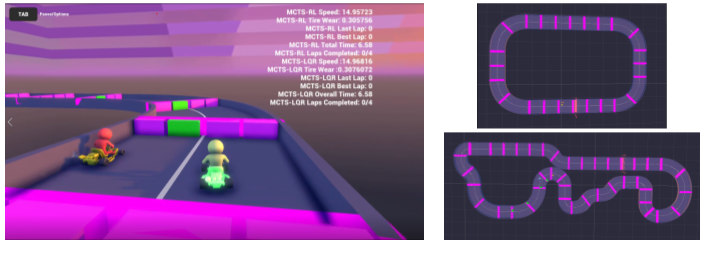
\includegraphics[width=\textwidth]{Figures/UnityEnvironment.png}
  \caption[Screenshots of Unity simulation environment] {Kart racing environment from a racer's perspective (left), a bird's eye view of the oval track (right-top), and the complex track (right-bottom) in the Unity environment. The purple boxes visualize the lanes across checkpoints along the track, and the highlighted green boxes show planned waypoints determined by the hierarchical controllers.}
  \label{fig:experiment_tracks}
\end{figure}
\section{Head-to-Head Racing Results}
% Two Tracks, 50 races head to head each
Our experiments include head-to-head racing on a basic oval track (which the learning-based agents were trained on) and a more complex track shown in Figure \ref{fig:experiment_tracks}. Specifically, the complex track involves challenging track geometry with turns whose radii change along the curve, tight U-turns, and turns in both directions. To be successful, the optimal racing strategy requires some understanding of the shape of the track along a sequence of multiple turns. Every pair of controllers competes head-to-head in 100 races on both tracks. The dynamical parameters (cornering limitations, top speed, acceleration, braking, etc.) of each player's vehicle are identical, and the players start every race at the same initial checkpoint. The only difference in their initial states is the lane in which they start. In order to maintain fairness with respect to starting closer to the optimal racing line, we alternate the starting lanes between each race for the players.

Our experiments primarily seek to identify the importance of hierarchical game-theoretic reasoning and the strength of MCTS as a high-level planner for racing games. We count the number of wins against each opponent, average collisions-at-fault per race, average illegal lane changes per race, and a safety score (a sum of the prior two metrics) for the controllers. Appendix \ref{app:hier_results} provides the complete results with all of the metrics collected. We also provide a video\footnote{\vidurl} demonstrating them in action. 
\begin{figure} [H]
  \centering
  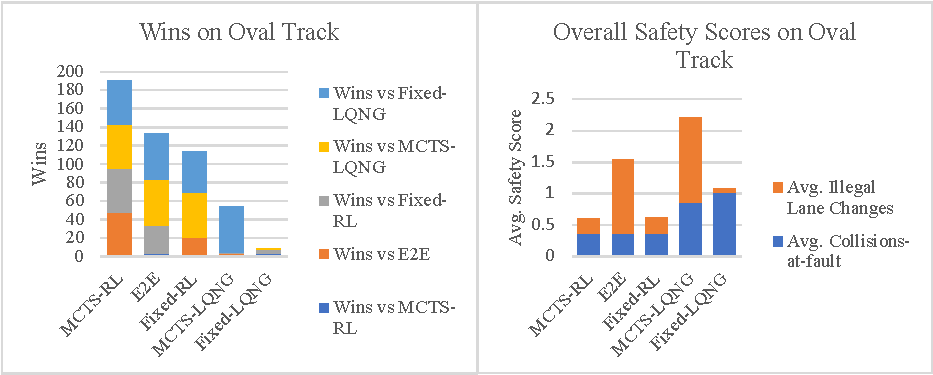
\includegraphics[width=\textwidth]{Figures/OvalResultsNew2.pdf}
  \caption{Results from head-to-head racing on the oval track.}
  \label{fig:results_oval}
  \bigskip
  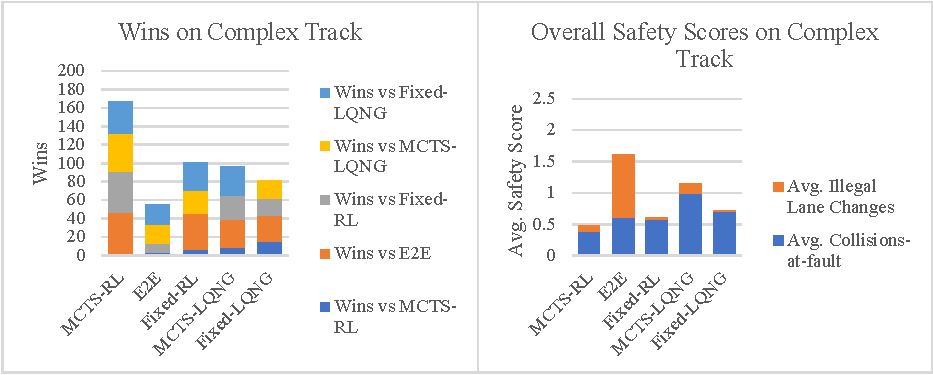
\includegraphics[width=\textwidth]{Figures/ComplexResultsNew2.pdf}
  \caption{Results from head-to-head racing on the complex track.}
  \label{fig:results_complex}
\end{figure}

Based on the plots in Figures \ref{fig:results_oval} and \ref{fig:results_complex}, we conclude the following key points:

\begin{enumerate}[wide, labelindent=0pt]
% MCTS-based variants outperformed respective baselines
\item \textbf{The proposed hierarchical variants outperformed their respective baselines.} 

The results amongst MCTS-RL, Fixed-RL, and E2E show the effectiveness of our hierarchical structure. While all three of the MARL-based agents were only trained on the oval track, the MCTS-RL agent won the most head-to-head races while also maintaining the best safety score by better adapting its learning. Comparing the baselines against each other, Fixed-RL also has more wins and a better safety score than E2E aggregated across both tracks. This result indicates that some type of hierarchical structure is favorable. It suggests that a straightforward task of trajectory tracking is much easier to learn for a deep neural network than having to learn both strategic planning and respect for the safety and fairness rules. 

Next, we compare MCTS-LQNG and Fixed-LQNG. Although MCTS-LQNG has a worse safety score, it has twice as many head-to-head wins when aggregated over both tracks. Furthermore, the main difference in their safety score is attributed to the fact that MCTS-LQNG considers multiple trajectories whereas Fixed-LQNG only follows a fixed trajectory that does not involve changing lanes often. Their collision-at-fault numbers, aggregated from both tracks, are similar. Furthermore, MCTS-LQNG was more competitive in its races against E2E and Fixed-RL on the complex track while the Fixed-LQNG had about 9\% fewer wins in the races against them combined. MCTS-LQNG considered trajectories that could result in overtakes when opponents made mistakes from any part of the track. However, to overtake, Fixed-LQNG had to rely on opponents making mistakes that were not along its fixed trajectory.  

% RL is better than LQNG for low-level
\item \textbf{MARL is more successful and robust than LQNG as a low-level planner.}  

In both tracks, the MARL-based agents outperformed their LQNG-based counterparts in terms of the two key metrics: head-to-head wins and safety scores. However, this result is likely due to the heuristic simplifications in our LQNG design. Vehicle dynamics are only linearized around the initial state of each agent and are time-invariant, meaning the linear approximation is only valid for a very short time horizon. Therefore, LQNG-based controllers could only rely on braking/acceleration instead of yaw-rate to avoid collisions, thus often conceding in close battles and losing races. If the dynamics were linearized over the state at each timestep $t$ instead of just the initial state at $t_0$, we could use a larger time horizon and expect better performance for the LQNG-based agents. The difference in safety scores primarily arises from increased illegal lane changes by these agents. The high-level planner runs in parallel with the low-level and at a lower frequency. As a result, the calculated high-level plan is sometimes delayed and does not account that the low-level controllers have already made choices that might contradict the initial steps in the plan. It causes the LQNG-based controllers to more often break the lane changing rules by swerving across the track to immediately follow the high-level plan when it is updated. The MARL-based agents are more robust to this situation because they have those safety rules encoded in their reward structures, albeit with smaller weights. 

% MCTS-RL is the best overall controller.
\item \textbf{MCTS-RL outperforms all other implemented controllers.}  

 MCTS-RL has the best safety score and recorded a win rate of over 88\% of the 400 head-to-head races it participated in across both tracks. It combined the advantage of having a high-level planner that evaluates long-term plans and a low-level planner that is robust to the possibility that the high-level plans may be out of date. For example, Figure~ \ref{fig:mctsrl:overtake} demonstrates how the high-level planner provided a long-term strategy, guiding the agent to give up an advantage at present for a greater advantage in the future when overtaking. The RL-based low-level planner approximately follows the high-level strategy in case stochasticity of the MCTS algorithm yields a waypoint that seems out of place (e.g., the checkpoint between $t=3$ and $t=4$ in Figure~ \ref{fig:mctsrl:overtake}). Furthermore, MCTS-RL is also successful at executing defensive maneuvers as seen in Figure~ \ref{fig:mctsrl:defense} due to those same properties of long-term planning and low-level robustness. Both of these tactics resemble strategies of expert human drivers in real head-to-head racing.
 \end{enumerate}
 
 \begin{sidewaysfigure}
  \centering
  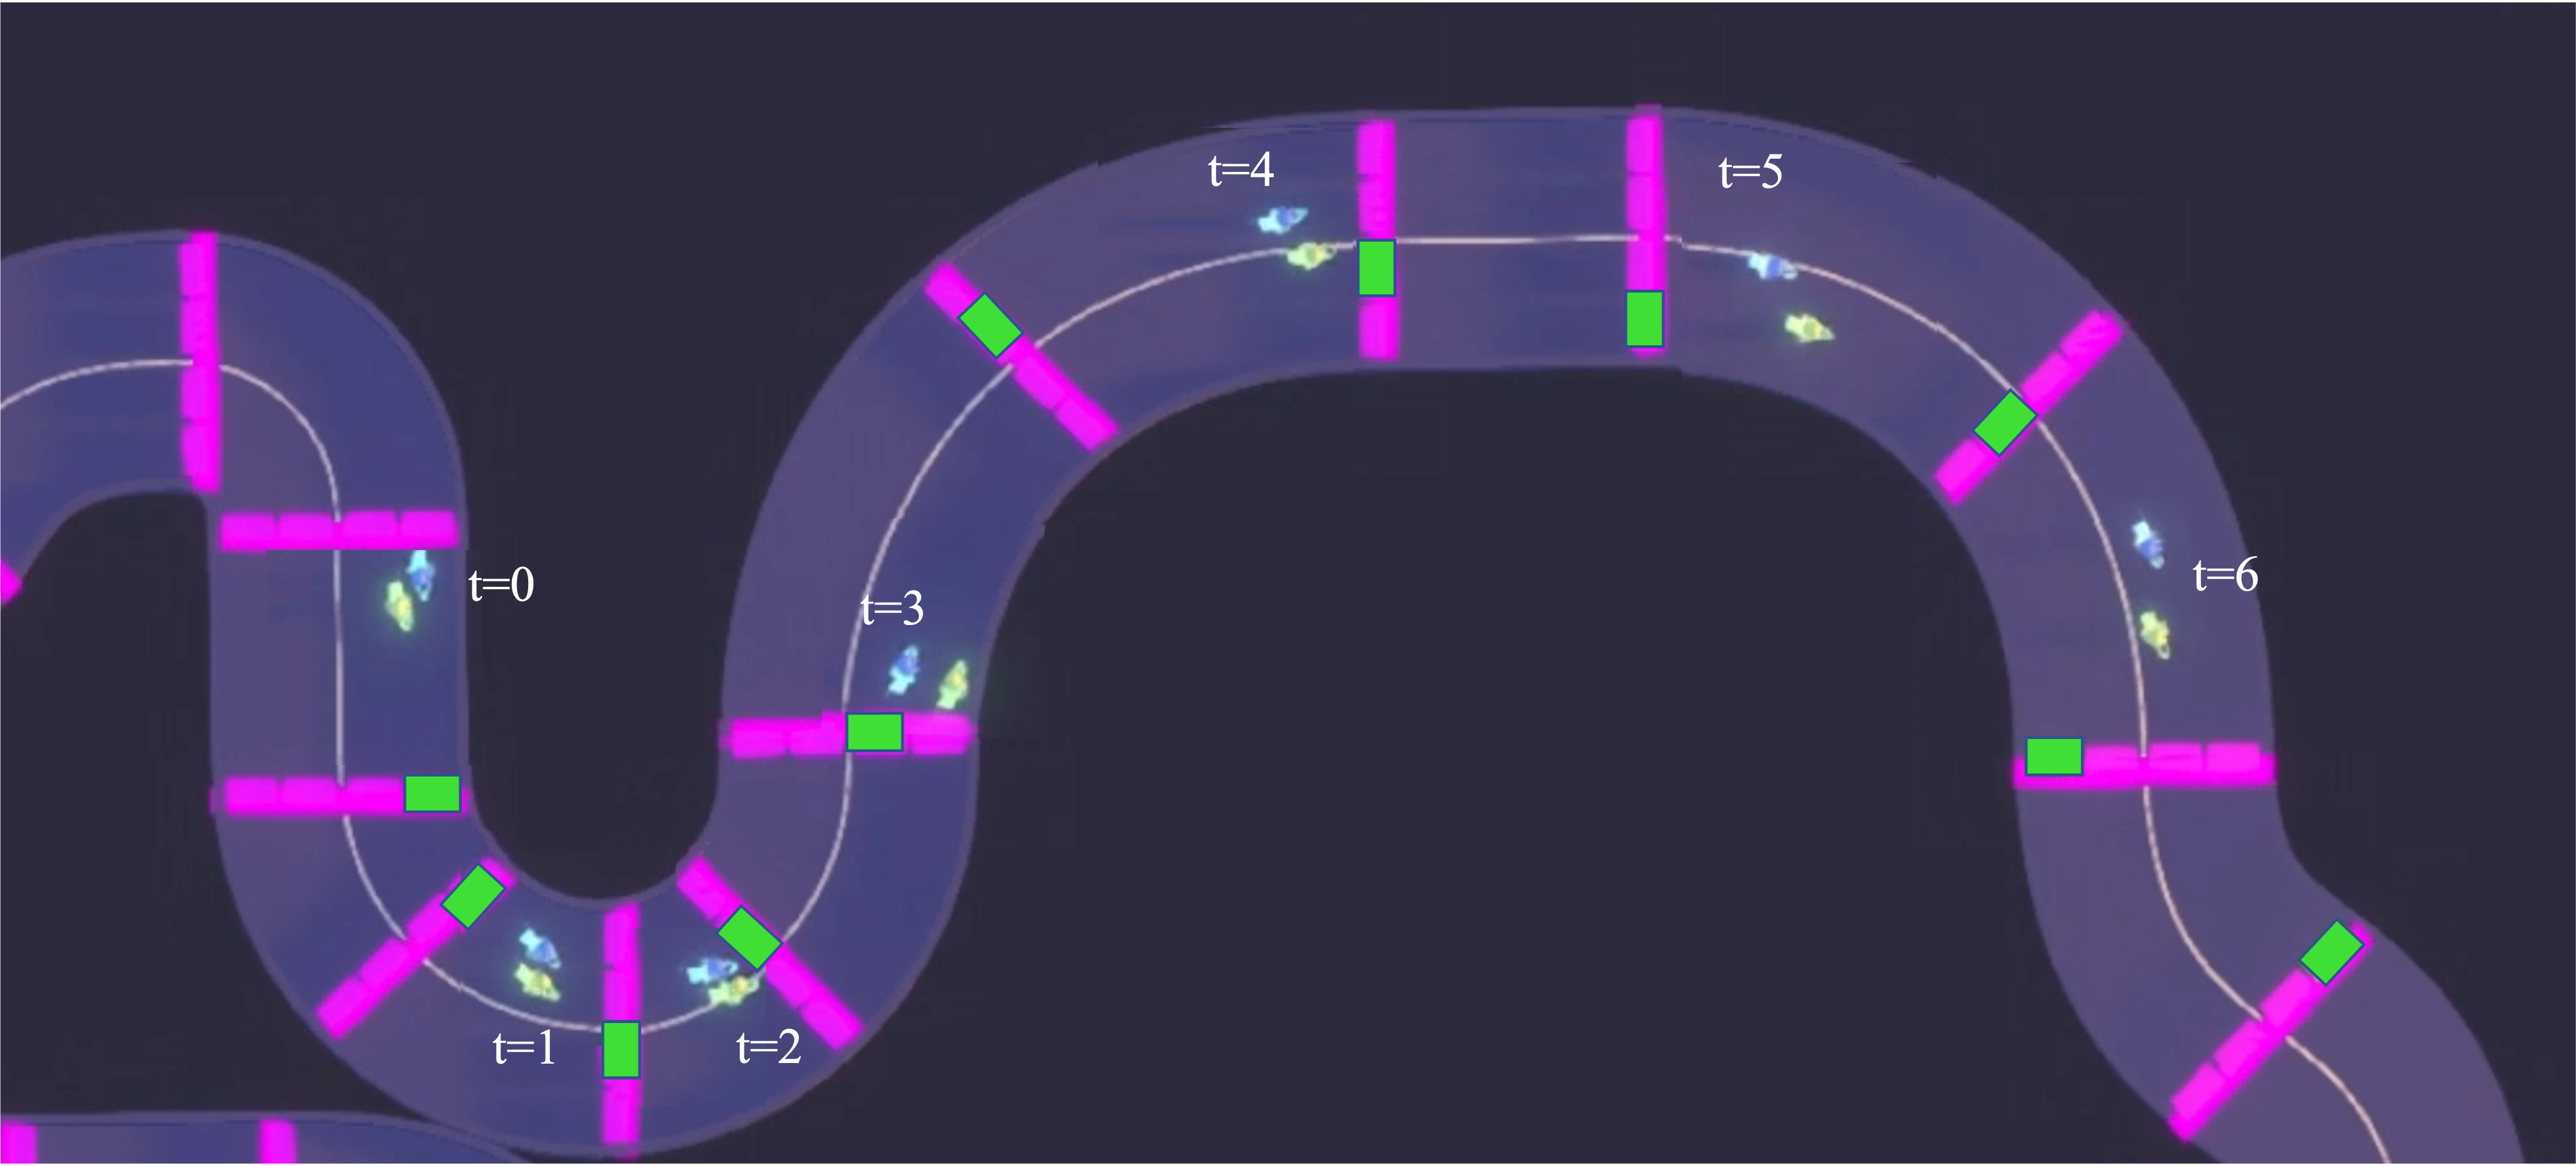
\includegraphics[width=\textwidth]{Figures/MCTSRLOvertake.png}
  \caption [Overtaking maneuver by MCTS-RL controller.] {An overtaking maneuver executed by the MCTS-RL agent (green) against the E2E agent (blue) on the complex track. Notice how, from $t=0$ to $t=2$, the MCTS-RL agent gives up a slight advantage and takes a wider racing line on the first turn. However, the exit of the wide racing line of the first turn places the MCTS-RL agent at the inside of the next two turns where it is able to gain an even greater advantage when passing the E2E agent from $t=3$ to $t=6$. The green boxes along each checkpoint also highlight the long-term plan calculated by the MCTS planner for this tactic.}
  \label{fig:mctsrl:overtake}
\end{sidewaysfigure}
\begin{figure} [H]
    \centering
  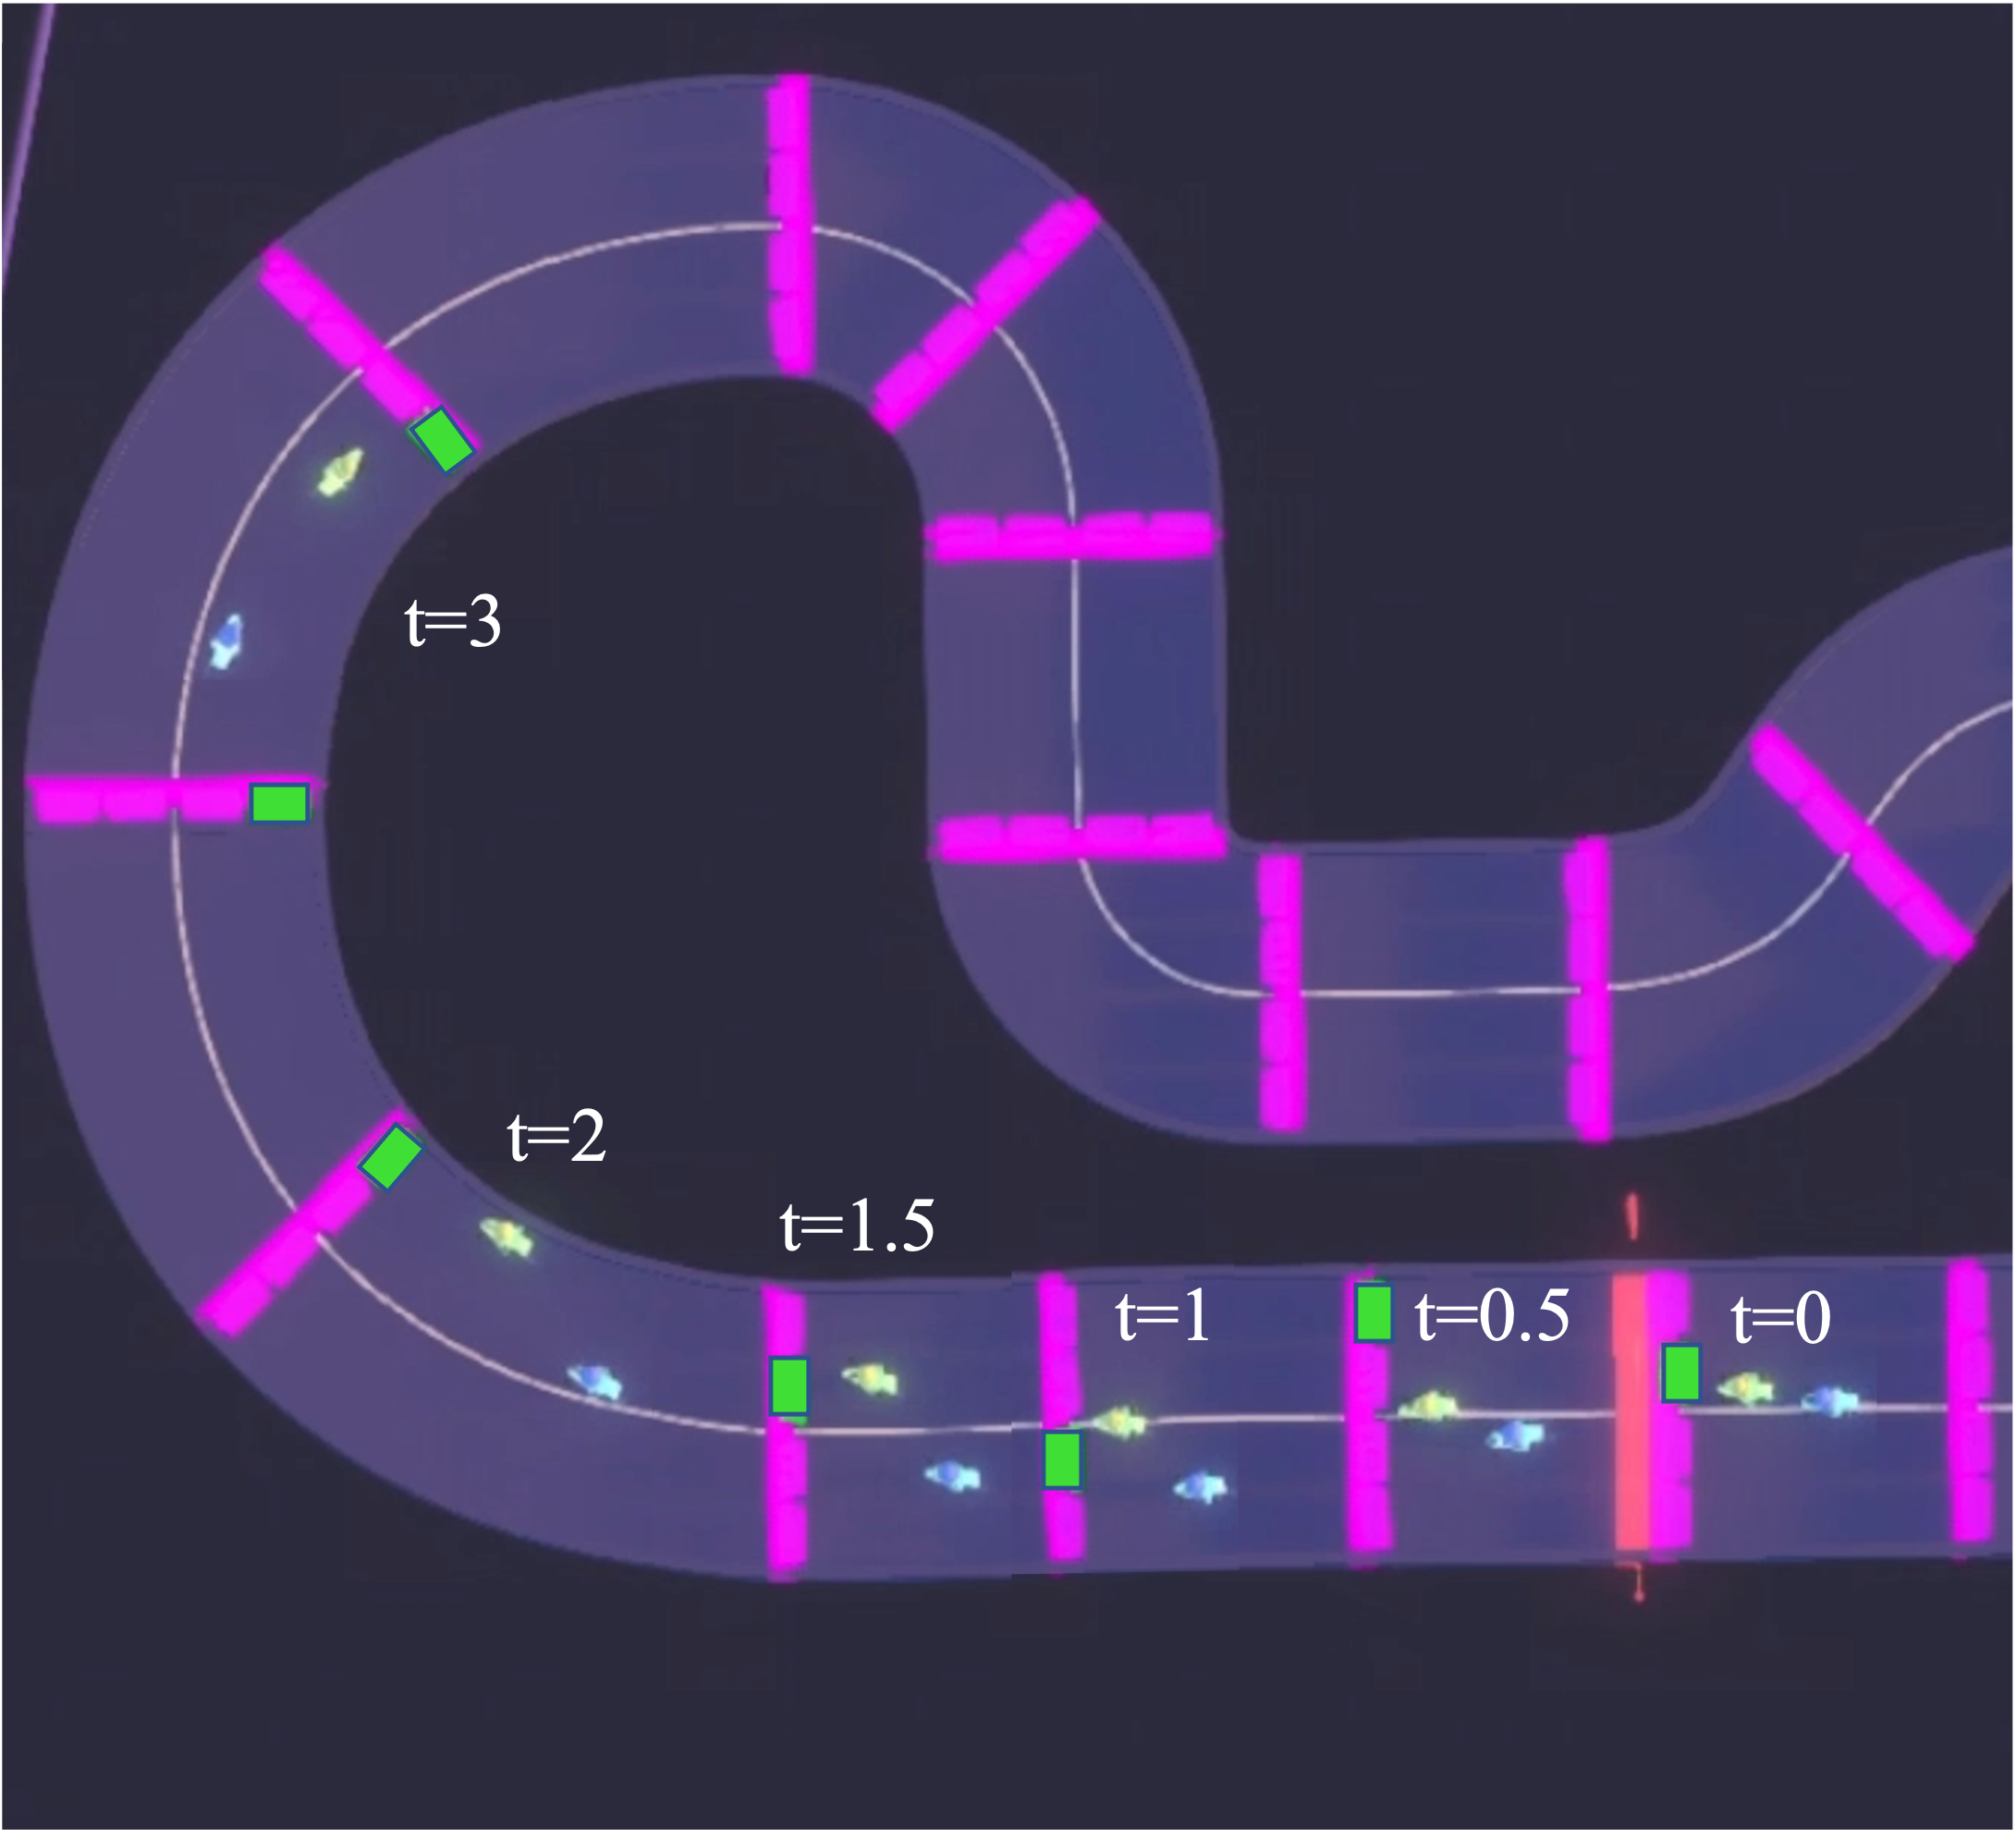
\includegraphics[width=0.7\textwidth]{Figures/MCTSRLDefense.png}
  \caption[Defensive maneuver by MCTS-RL controller.]{A defensive maneuver executed by the MCTS-RL agent (green) against the E2E agent (blue) on the complex track.  Before reaching the turn, the MCTS planner calculates to switch lanes to the left first ($t=0$ to $t=1$) and then move to the right for the inside of the turn. This motion forces the E2E agent to make an evading move to avoid collision and take an even wider turn, thus increasing the overall gap at the end. The green boxes along each checkpoint highlight the long-term plan calculated by the MCTS planner for this tactic.}
  \label{fig:mctsrl:defense}
\end{figure}